%%%%% Document Setup %%%%%%%%

\documentclass[12pt, onecolumn]{revtex4}    % Font size (12pt) and column number (one or two).

\usepackage[a4paper, left=2.5cm, right=2.5cm, top=2.5cm, bottom=2.5cm]{geometry}  % Defines paper size and margin length

\renewcommand{\baselinestretch}{1}     % Defines the line spacing

\usepackage{subcaption}

\usepackage[font=small, labelfont=bf]{caption}                      % Defines caption font size and caption title bolded
\captionsetup[figure]{justification=justified, singlelinecheck=off, font=footnotesize} 
\captionsetup{compatibility=false}

\usepackage{graphics,graphicx,epsfig,ulem}	% Makes sure all graphics works
\usepackage{amsmath} 						% Adds mathematical features for equations

\usepackage{etoolbox}                       % Customise date to preferred format
\makeatletter
\patchcmd{\frontmatter@RRAP@format}{(}{}{}{}
\patchcmd{\frontmatter@RRAP@format}{)}{}{}{}
\renewcommand\Dated@name{}
\makeatother

\usepackage[UKenglish]{babel}% http://ctan.org/pkg/babel

\usepackage{fancyhdr}

\pagestyle{fancy}                           % Insert header
\renewcommand{\headrulewidth}{0pt}
\lhead{\small Z0962251}  

\def\thesection{\arabic{section}}
\def\thesubsection{\alph{subsection}}

\def\bibsection{\section*{References}}        % Position reference section correctly
\setcitestyle{authoryear,round}
\setlength\bibhang{0.2in}
\usepackage[colorlinks]{hyperref}
\hypersetup{
    colorlinks=true,
    linkcolor=black,
    citecolor=black,    
    urlcolor=black,
}

%%%%% Document %%%%%
\begin{document}                     


\title{The measurement of the Hubble Constant: beyond the cosmic ladder} 
\date{Submitted: \today{}}
\author{Z0962251}

\maketitle
\thispagestyle{plain} % produces page number for front page

A precisely determined Hubble's constant $H_0$ would have an overarching effect on any feature of cosmological theory: the age of the Universe, the critical density of the Universe, or in the formation of cosmic structure. Producing a conclusive value for $H_0$ is difficult as absolute distances on the cosmic scale are difficult to measure. Inhomogeneous gravitational acceleration generates motion which does not follow the simple expansion as described by Hubble's Law $v=H_0 d$. An uncertainty arises due to the discrepancy between the methods to connect local distances to the smooth large-scale Hubble flow \citep{fukugita_cosmic}. \\

Several approaches for cosmic distance measurement should therefore be used to reduce systematic errors. These measurements can form the ``rungs'' of a \textit{cosmic distance ladder}, where large extragalactic distances ($>1000$ Mpc) are informed and calibrated by techniques which have smaller ranges \citep{carroll_astro}. Astronomers may employ a variety of methods in tandem, therefore the ladder could instead be expressed as several pathways (Figure \ref{fig:cosmic_pathways}). 

% words: 154

\begin{center}
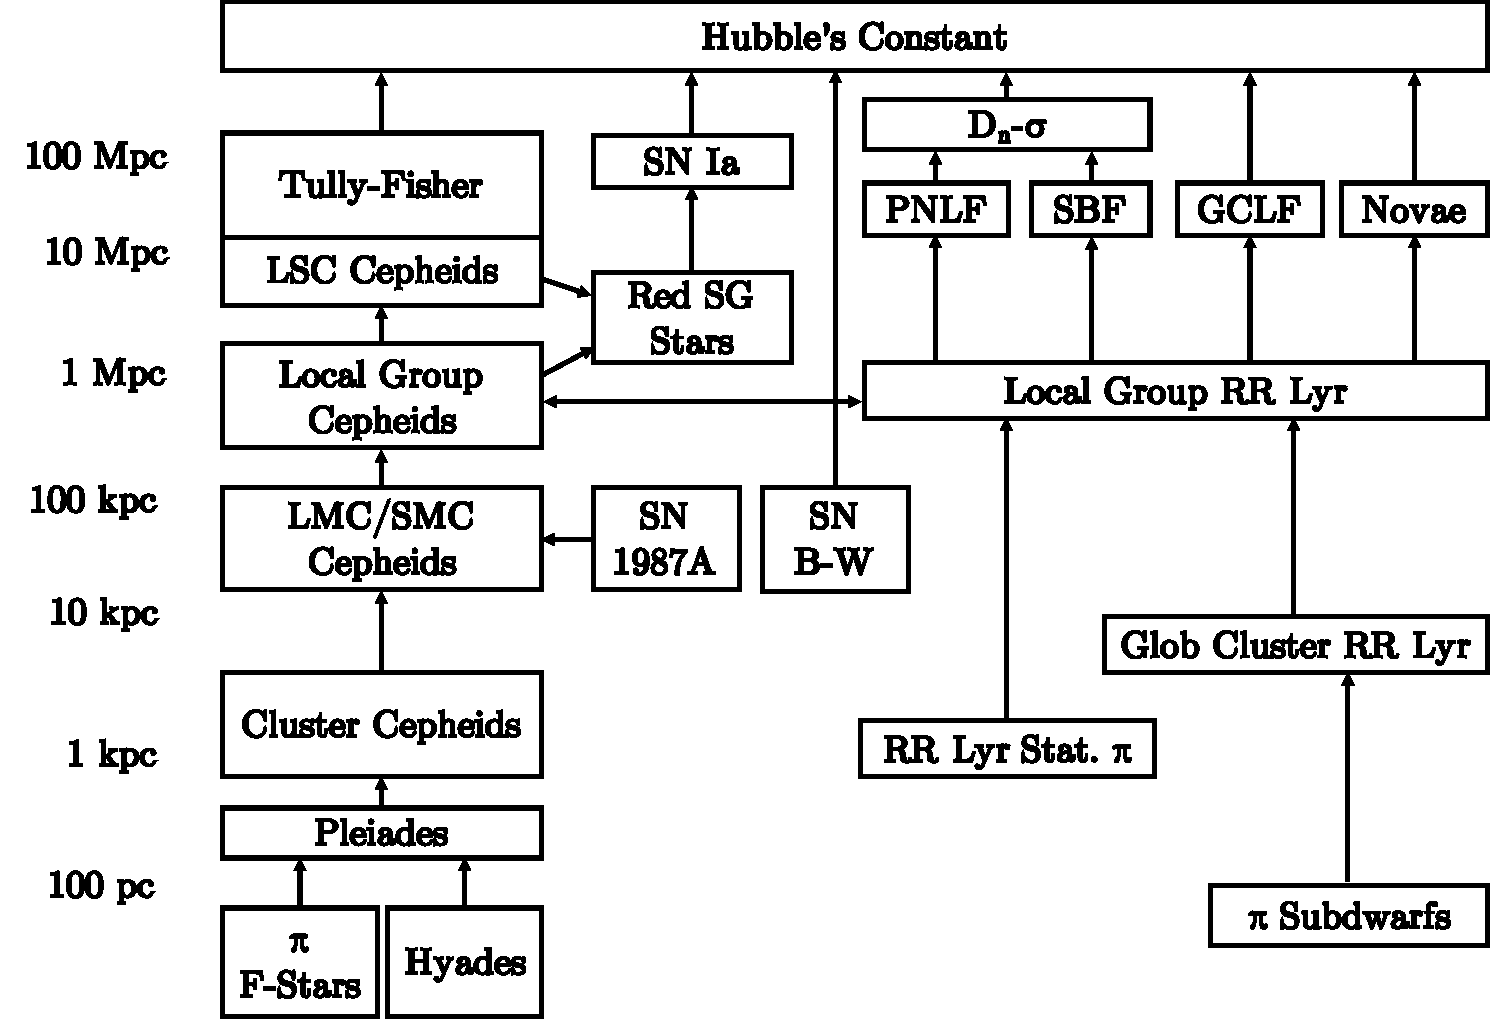
\includegraphics[width=0.8\linewidth]{figures/cosmic_distance_pathways}
\captionof{figure}[Cosmic Distance Pathways]{Adapted from \cite{jacoby_extragal}, this diagram illustrates the various approaches to calculate $H_0$, each technique is roughly placed at the approximate range it operates at. One can see that there is not one strict ``cosmic ladder'', rather multiple pathways. For reference, the acronyms used are: B-W - Baade-Wessenlink; GCLF - Globular-Cluster Luminosity Function; LSC - Local Super Cluster; PNLF - Planetary Nebula Luminosity Function; SBF - Surface-Brightness Fluctuations; SG - Super Giant; SN - Supernovae; $\pi$ - parallax.}
\label{fig:cosmic_pathways}
\end{center}

The Hubble Space Telescope (HST) $H_0$ Key Project was an effort in the early 2000s to determine $H_0$ by calculating distances to Cepheid variables in local galaxies ($\le 20$ Mpc) then applying them as a calibration to 5 secondary independent distance indicators. Described by \cite{freedman_hstkeystone}, four of the methods (Type Ia supernovae, Tully-Fisher relation, surface-brightness fluctuations, and Type II supernovae) were able to produce $70\le H_0 \le72$ kms$^{-1}$ Mpc$^{-1}$ and the remaining technique (fundamental plane for elliptical galaxies) $H_0\approx82$ kms$^{-1}$ Mpc$^{-1}$. Over the next decade, the methodology would be refined and the sample of Cepheids and Type Ia supernovae would increase leading to $H_0=73.8 \pm2.4$ kms$^{-1}$ Mpc$^{-1}$ \citep{2011ApJ...730..119R}. These results set a standard benchmark for $H_0$, they were found by taking steps along the cosmic ladder and whilst they have high accuracy, it would be beneficial to directly calculate $H_0$ at large distances without the need to calibrate with Cepheids. \\

% words: 140

One of the key alternative methods is the usage of Cosmic Microwave Background (CMB) measurements. 

% CMB measurements: Planck and WMAP

% Sunyaev–Zel'dovich effect and Chandra X-ray

% Gravitational lensing

% Gravitational waves

\newpage

\bibliographystyle{agsm}

%\nocite{fukugita_cosmic}
%\nocite{carroll_astro}
%\nocite{jacoby_extragal}
\bibliography{cosmic_ladder}

\newpage

\end{document}